%%% SOME NOTES ON THE NONLINEAR PENDULUM
\documentclass{tjwNOTES}

%%% TITLE
\title{The Nonlinear Pendulum}
\author{Dr Timothy J. Walton}
\date{\today}
\pagestyle{headings}

%%% PACKAGE
\usetikzlibrary{intersections, pgfplots.fillbetween}

%%% COMMANDS


%%%%%%%%%%%%%%%%%%%%%%%%%%%%%%%%%%%%%%%%%%%%%%%%%%%%%%%%%%%%%%%%%%%%%%%%
\begin{document}
%%%%%%%%%%%%%%%%%%%%%%%%%%%%%%%%%%%%%%%%%%%%%%%%%%%%%%%%%%%%%%%%%%%%%%%%
\maketitle

Consider the motion of a pendulum: a material point of mass $m$ suspended on an inextensible string of length $L$: 
\begin{center}
	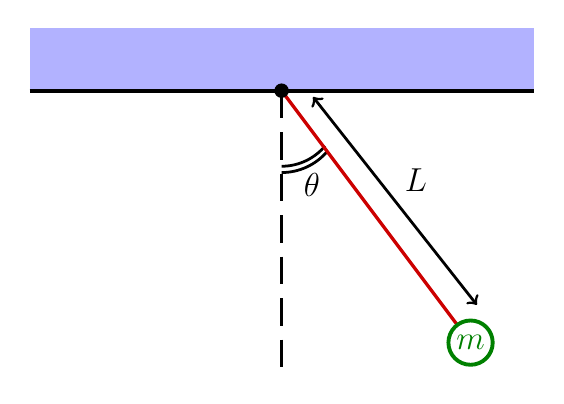
\begin{tikzpicture}[scale=0.8]
		\fill[blue!30!white] (0,0) rectangle (8,1);
		\draw[black, line width=1pt] (4,-1.2) arc (-90:-40:0.9cm);
			\draw[black, line width=1pt] (4,-1.3) arc (-90:-40:0.95cm);
			\node[right] at (4.2,-1.5) {\mbox{\large$\pmb{\theta}$}};
		\draw[black,line width=1.4pt] (0,0) -- (8,0);
		\draw[black,line width=1pt, dashed, dash pattern={on 10pt off 5pt}] (4,0) -- (4,-4.5);
		\draw[red!80!black, line width=1.2pt] (4,0) -- (7,-4);
			\draw[black, line width=1pt, <->] (4.5,-0.1) -- (7.1,-3.4) node[pos=0.4,right, xshift=0.2cm] {\mbox{\large $\pmb{L}$}};
		\draw[black, fill=black] (4,0) circle (3pt);
		\draw[green!50!black, fill=white, line width=1.4pt] (7,-4) circle (10pt); 
			\node[green!50!black] at (7,-4) {\mbox{\large $\pmb{m}$}};
	\end{tikzpicture}
\end{center}
Newton's second law\footnote{Consider tangential forces: $F=-mg\sin(\,\theta(t)\,)$ due to the weight of the mass. } yields an equation of motion of the pendulum in terms of the angular displacement $\theta(t)$:
\begin{align*}
	\left\{	\begin{array}{rl}
				\ddot{\theta}(t) + \omega^{2}\sin(\,\theta(t)\,) &\!=\; 0  \\[0.2cm]
				\theta(0) &\!=\; \theta_{0}\in\RR \\[0.2cm]
				\dot{\theta}(0) &\!=\; 0
			\end{array}\right.
\end{align*}
where, for simplicity, we have considered the initial angular velocity $\dot{\theta}(t)$ of the pendulum to be zero (i.e. the pendulum is dropped from rest) and we have defined
\begin{align*}
	\omega\,\equiv\,\sqrt{\frac{g}{L}}.
\end{align*}
Note that values of $\theta_{0},\theta(t)$ must lie in the interval $[-\pi/2,\pi/2]$. \\

To solve the ODE, we multiply by $\dot{\theta}(t)$:
\begin{align*}
	\dot{\theta}(t)\,\ddot{\theta}(t) + \omega^{2}\dot{\theta}(t)\,\sin(\,\theta(t)\,) \,=\, \frac{d}{dt}\left[ \frac{1}{2}\dot{\theta}(t)^{2} - \omega^{2}\cos(\,\theta(t)\,) \right] \,=\, 0
\end{align*}
using the chain rule. Integrating this equation over $[0,t]$ yields:
\begin{align*}
	\left[\frac{1}{2}\dot{\theta}(t)^{2} - \omega^{2}\cos(\,\theta(t)\,) \right]_{0}^{t} \,=\, 0 &\qLRA \frac{1}{2}\dot{\theta}(t)^{2} - \omega^{2}\cos(\,\theta(t)\,) + \omega^{2}\cos(\theta_{0})  \,=\, 0 \\[0cm]
	&\qLRA \dot{\theta}(t)^{2} \,=\, 2\omega^{2}\left[\df\cos(\,\theta(t)\,)-\cos(\theta_{0})\right].
\end{align*}
Using the double angle formula $\cos(\,\theta(t)\,)=1-2\sin^{2}(\theta(t)/2)$, we write:
\begin{align*}
	\cos(\,\theta(t)\,)-\cos(\theta_{0}) &\,=\, 1-2\sin^{2}(\theta(t)/2)-\cos(\theta_{0}) \,=\, \left(\df1-\cos(\theta_{0}\,)\right)\left( 1- \frac{2\sin^{2}(\theta(t)/2)}{1-\cos(\theta_{0})}\right)  \\[0cm]
		&\,=\, 2\sin^{2}(\theta_{0}/2)\left( 1- \frac{2\sin^{2}(\theta(t)/2)}{1-\cos(\theta_{0})}\right) \,=\, 2\sin^{2}(\theta_{0}/2)\left( 1- \frac{\sin^{2}(\theta(t)/2)}{\sin^{2}(\theta_{0}/2)}\right)  \\
		&\,=\, 2k\left( 1- \frac{\sin^{2}(\theta(t)/2)}{k^{2}}\right)
\end{align*}
where we have introduced the variable
\begin{align*}
	k \,\equiv\, \sin(\theta_{0}/2)
\end{align*}
and used $1-\cos(\theta_{0})=2\sin^{2}(\theta_{0}/2)$. Note the value of $k$ depends upon the initial condition and must lie in the interval $[0,\pi/4]$ (since $\theta\in[0,\pi/2]$). Thus, we have the differential equation:
\begin{align*}
	\dot{\theta}(t)^{2} \,=\, 4\omega^{2}k^{2}\left( 1- \frac{\sin^{2}(\theta(t)/2)}{k^{2}}\right) \qLRA \frac{\dot{\theta}(t)}{2k} \,=\, \omega\,\sqrt{ 1- \frac{\sin^{2}(\theta(t)/2)}{k^{2}} }.
\end{align*}
We wish to find the period of oscillation of the pendulum from this differential equation. We note from the initial conditions the pendulum is at an angle $\theta=\theta_{0}$ and at some (later) time, we must have $\theta=0$ when it passes the lowest point of its arc (we must now assume $\theta_{0}>0$). The time it takes the pendulum to travel between these two points is equivalent to one quarter of the time period, $T$. That is:
\begin{align*}
	\frac{T}{4} \,=\, \int_{\theta=0}^{\theta_{0}}\,\frac{dt}{d\theta}\,d\theta \qLRA T \,=\, 4\int_{\theta=0}^{\theta_{0}}\,\frac{d\theta}{\dot{\theta}(t)} \,=\, 4\int_{\alpha=0}^{\pi/2}\,\frac{d\alpha}{\dot{\alpha}(t)}.
\end{align*}
in terms of a new angle variable $\alpha(t)$ defined by:
\begin{align*}
	\sin(\,\alpha(t)\,) \,\equiv\, \frac{\sin(\theta(t)/2)}{k} \,=\, \frac{\sin(\theta(t)/2)}{\sin(\theta_{0}/2)}
\end{align*}
which, as $\theta(t)$ varies over the interval $[0,\theta_{0}]$, varies over $[0,\pi/2]$. Differentiating the relation with respect to $t$ gives:
\begin{align*}
	\dot{\alpha}(t)\,\cos(\,\alpha(t)\,) \,=\,\frac{\dot{\theta}(t)\,\cos(\theta(t)/2)}{2k} 
\end{align*}
or using $\cos(\theta(t)/2)=\sqrt{1-\sin^{2}(\theta(t)/2)}=\sqrt{1-k^{2}\sin^{2}(\,\alpha(t)\,)}$:
\begin{align*}
	\frac{\dot{\theta}(t)}{2k}  \,=\, \frac{\dot{\alpha}(t)\,\cos(\,\alpha(t)\,)}{\cos(\theta(t)/2)} \,=\,\frac{\dot{\alpha}(t)\,\cos(\,\alpha(t)\,)}{\sqrt{1-k^{2}\sin^{2}(\,\alpha(t)\,)}} .
\end{align*}
Thus, the differential equation becomes:
\begin{align*}
	\frac{\dot{\alpha}(t)\,\cos(\,\alpha(t)\,)}{\sqrt{1-k^{2}\sin^{2}(\,\alpha(t)\,)}} \,=\,\omega\,\sqrt{ 1- \sin^{2}(\,\alpha(t)\,) } \,=\, \omega\,\cos(\,\alpha(t)\,) 
\end{align*}
or after rearranging:
\begin{align*}
	\dot{\alpha}(t) \,=\, \omega\,\sqrt{ 1- k^{2}\sin^{2}(\,\alpha(t)\,)} .
\end{align*}
Hence the time period can be written:
\begin{align*}
	T \,=\, \frac{4}{\omega}\int_{\alpha=0}^{\pi/2}\,\frac{d\alpha}{\sqrt{ 1- k^{2}\sin^{2}(\alpha)}} \,=\, \frac{4\,K(k)}{\omega}
\end{align*}
in terms of the complete elliptic integral of the first kind $K$ with modulus $k$. Recall that $k\in(0,\pi/4)$ which is a valid parameter range for the elliptic integral and implies the integrand will not go singular. Since the (generalised binomial) series\footnote{Here we use the generalised binomial coefficients $\ds \binom{\alpha}{k}=\frac{\alpha(\alpha-1)\cdots(\alpha-k+1)}{k(k-1)\cdots 1}=\prod_{i=1}^{k}\frac{\alpha-i+1}{i}$.}
\begin{align*}
	\frac{1}{\sqrt{1-x}} &\,=\, (1-x)^{-\frac{1}{2}} \,=\, \sum_{j=0}^{\infty}\binom{-1/2}{j}\,(-x)^{j} \,=\, 1+\sum_{j=1}^{\infty}\binom{-1/2}{j}\,(-x)^{j}\\[0.2cm]
	& \,=\, 1+\sum_{j=1}^{\infty}(-1)^{j}\left(\prod_{i=1}^{j}\frac{1/2-i}{i}\right)\,x^{j} \,=\, 1+\sum_{j=1}^{\infty}(-1)^{j}\left(\prod_{i=1}^{j}\frac{1-2i}{2i}\right)\,x^{j} 
\end{align*}
is convergent\footnote{This series converges absolutely on $(0,1)$ and uniformly on $(0,\rho]$ for $0<\rho<1$ by the Weierstrass M-test.} for $x\in(0,1)$, we may write
\begin{align}\label{SQRTseries}
	\frac{1}{\sqrt{1-k^{2}\sin^{2}(\alpha)}} \,=\, 1+\sum_{j=1}^{\infty}(-1)^{j}\left(\prod_{i=1}^{j}\frac{1-2i}{2i}\right)\,k^{2j}\sin^{2j}(\alpha)
\end{align}
since $k^{2}\sin(\alpha)\in(0,\pi^{2}/16)\subset(0,1)$ for all $\alpha$. Furthermore
\begin{align*}
	\int_{\alpha=0}^{\pi/2}\sin^{2n}(\alpha)\,d\alpha &\,=\, \left(\frac{2n-1}{2n}\right)I_{2n-2} \,=\, \left(\frac{2n-1}{2n}\right)\left(\frac{2n-3}{2n-2}\right)I_{2n-4} \,=\, \left(\frac{2n-1}{2n}\right)\left(\frac{2n-3}{2n-2}\right)\cdots\left(\frac{1}{2}\right)I_{0} \\[0.2cm]
		&\,=\,\frac{\pi}{2} \prod_{k=1}^{n}\frac{2k-1}{2k} 
\end{align*}
using the reduction formula\footnote{The reduction formula can be proved by a simple application of integration by parts} 
\begin{align*}
	I_{n} \,\equiv\, \int_{\alpha=0}^{\pi/2}\sin^{n}(\alpha)\,d\alpha \,=\, \left(\frac{n-1}{n}\right)I_{n-2}, \qquad I_{0} \,=\, \int_{\alpha=0}^{\pi/2}\,d\alpha \,=\, \frac{\pi}{2}.
\end{align*}
Thus, due to the uniform convergence\footnote{This permits us to interchange summation and integration.} of the series (\ref{SQRTseries}), we have a power series expansion of the complete elliptic integral of the first kind:
\begin{align*}
	K(k) &\,=\, \int_{\alpha=0}^{\pi/2}\,\frac{d\alpha}{\sqrt{ 1- k^{2}\sin^{2}(\alpha)}} \,=\, \int_{\alpha=0}^{\pi/2}\,\left(1+\sum_{j=1}^{\infty}(-1)^{j}\left(\prod_{i=1}^{j}\frac{1-2i}{2i}\right)\,k^{2j}\sin^{2j}(\alpha)\right)d\alpha \\[0.2cm]
	&\,=\, \int_{\alpha=0}^{\pi/2}d\alpha + \sum_{j=1}^{\infty}(-1)^{j}\left(\prod_{i=1}^{j}\frac{1-2i}{2i}\right)\,k^{2j}\int_{\alpha=0}^{\pi/2}\sin^{2j}(\alpha)d\alpha \\[0.2cm]
	&\,=\, \frac{\pi}{2} + \sum_{j=1}^{\infty}(-1)^{j}\left(\prod_{i=1}^{j}\frac{1-2i}{2i}\right)\,k^{2j}\cdot\left(\frac{\pi}{2} \prod_{i=1}^{j}\frac{2i-1}{2i}\right) \\[0.2cm]
	&\,=\, \frac{\pi}{2} + \frac{\pi}{2}\sum_{j=1}^{\infty}\left(\prod_{i=1}^{j}(-1)\right)\left(\prod_{i=1}^{j}\frac{1-2i}{2i}\right)\left(\prod_{i=1}^{j}\frac{2i-1}{2i}\right)k^{2j} \,=\, \frac{\pi}{2}\left[1+\sum_{j=1}^{\infty}\left(\prod_{i=1}^{j}\frac{2i-1}{2i}\right)^{2}\,k^{2j} \right].
\end{align*}
It can be checked (using the ratio test, for example) that the series in the expansion above converges absolutely for all $k\in[0,1)$. Thus, we may write the time period of our pendulum as
\begin{align*}
	T &\,= \frac{4K(k)}{\omega}K \,=\, \frac{2\pi}{\omega}\left[1+\sum_{j=1}^{\infty}\left(\prod_{i=1}^{j}\frac{2i-1}{2i}\right)^{2}\,k^{2j} \right]
\end{align*}
or, after restoring variables and expanding:
\begin{align*}
	T &\,= 2\pi\sqrt{\frac{L}{g}}\left[1 + \sum_{j=1}^{\infty}\left(\prod_{i=1}^{j}\frac{2i-1}{2i}\right)^{\!2}\,\sin^{2j}\left(\frac{\theta_{0}}{2}\right)\right]
\end{align*}
using $\omega=\sqrt{g/L}$ and $k=\sin(\theta_{0}/2)$. We recognise the first term as the known formula for the period of a pendulum with small oscillations. 




%%%%%%%%%%%%%%%%%%%%%%%%%%%%%%%%%%%%%%%%%%%%%%%%%%%%%%%%%%%%%%%%%%%%%%%%%%%%%%%%%%%%%%%%%%%%%%
\end{document}
